\documentclass{report}
\usepackage[table,xcdraw]{xcolor}
\usepackage{tikz}
\usepackage{fancyhdr}
\usepackage[utf8]{vietnam}
\usepackage{hyperref} % Hyperlink
\usepackage{parskip}
\usepackage[left=2cm,right=2cm,top=2cm,bottom=2cm]{geometry}
\usetikzlibrary{calc}
\usepackage{titlesec} % Change section font
\usepackage{multirow}
\usepackage{graphicx}
\usepackage{algorithm,algorithmic}
\usepackage{multicol}
\usepackage{setspace}
\usepackage{pdfpages}
\usepackage{lscape}
\usepackage{subfigure}
\usepackage{tabularray}
\usepackage{amsmath}
\usepackage{indentfirst}

% ========== [LANGUAGE] ==========
\def\lang{1} % 0 == English, 1 == Vietnamese

\ifnum\lang = 0
    \usepackage[english]{babel}
\fi
% ========== END OF [LANGUAGE] ==========





\begin{document}

% ========== [TITLE PAGE] ==========
\begin{titlepage}

\begin{tikzpicture}[overlay,remember picture]
\draw[line width=4pt]
    ($ (current page.north west) + (1cm,-1cm) $)
    rectangle
    ($ (current page.south east) + (-1cm,1cm) $);
\draw[line width=1.5pt]
    ($ (current page.north west) + (1.2cm,-1.2cm) $)
    rectangle
    ($ (current page.south east) + (-1.2cm,1.2cm) $);
\end{tikzpicture}


\begin{center}
% Upper part of the page
\ifnum\lang = 0
    \textbf{\Large UNIVERSITY OF SCIENCE}\\[0.2cm]
    \textbf{\Large FACULTY OF INFORMATION TECHNOLOGY}\\
\else
    \textbf{\Large TRƯỜNG ĐẠI HỌC KHOA HỌC TỰ NHIÊN}\\
    \textbf{\Large KHOA CÔNG NGHỆ THÔNG TIN}\\
\fi

% University Logo
\begin{figure}[!h]
    \centering
    
\includegraphics[width=8cm, height=8cm]{assets/KHTN.png}
\end{figure}

% Title
\rule{\textwidth}{1pt} \\[0.4cm]
{\huge \bfseries BÁO CÁO ĐỒ ÁN - LINEAR REGRESSION}\\[0.4cm]
\textsc{\Large TOÁN ỨNG DỤNG VÀ THỐNG KÊ}
\rule{\textwidth}{1pt} \\[2cm]

% Student name
\begin{center}
    \textbf{\Large HỌ VÀ TÊN: BÙI ĐỖ DUY QUÂN}\\[0.5cm]
    \textbf{\Large MÃ SỐ SINH VIÊN: 21127141}\\[0.5cm]
    \textbf{\Large LỚP: 21CLC02}\\[2cm]
\end{center}

% Advisor name
\begin{center}
    \ifnum\lang = 0
        \textbf{\Large Lecturers: \\[0.2cm]}
    \else
        \textbf{\Large Giảng viên hướng dẫn: \\[0.2cm]}
    \fi
    \Large{Phan Thị Phương Uyên}
\end{center}
\vfill

% Bottom of the page
\ifnum\lang = 0
    \selectlanguage{english} 
\fi
{\large \today}
\end{center}
\end{titlepage}
% ========== END [TITLE PAGE] ==========





% ========== [HEADER AND FOOTER] ==========
\pagestyle{fancy}
\setlength{\headheight}{0.5cm}
\fancyhf{}
\lhead{\textbf{Đồ án 03}}
\rhead{\textbf{Toán ứng dụng và thống kê}}
\ifnum\lang = 0
    \rfoot{Page \thepage}
\else
    \rfoot{Trang \thepage}
\fi
% ========== END [HEADER AND FOOTER] ==========





% ========== [TABLE OF CONTENTS] ==========
\Large
\tableofcontents
\thispagestyle{fancy} % Fix footer and header
\vfill
\pagebreak
% ========== END [TABLE OF CONTENTS] ==========





% ========== [SECTION NUMBERING] ==========
\setcounter{secnumdepth}{10} % Section numbering depth 

\renewcommand\thesection{\arabic{section}} % Section start from 1,2,3...
\renewcommand\thesubsection{\thesection.\arabic{subsection}} % Subsection start from 1,2,3,...
\renewcommand\thesubsubsection{\alph{subsubsection}}
\titleformat{\paragraph}
{\normalfont\normalsize\bfseries}{\theparagraph}{1em}{}
\titlespacing*{\paragraph}
{0pt}{3.25ex plus 1ex minus .2ex}{1.5ex plus .2ex}

\titleformat*{\section}{\Large\bfseries}
\titleformat*{\subsection}{\Large\bfseries}
\titleformat*{\subsubsection}{\Large\bfseries}
% ========== END [SECTION NUMBERING] ==========





% ========== [MAIN CONTENT] ==========
\section{YÊU CẦU CỦA ĐỒ ÁN}
\begin{itemize} \label{sec:requirement}
    \item Xây dựng mô hình dự đoán \textbf{mức lương} của kỹ sư sử dụng \textbf{mô hình hồì quy tuyến tính (linear regression)} với các yêu cầu sau:
    \begin{enumerate}
        \item Sử dụng 11 đặc trưng gồm: \textbf{Gender, 10percentage, 12percentage, CollegeTier, Degree, collegeGPA, CollegeCityTier, English, Logical, Quant, Domain}
    
        \item Sử dụng 5 đặc trưng tính cách: \textbf{conscientiousness, agreeableness, extraversion, nueroticism, openess\_to\_experience} và sử dụng phương pháp \textbf{k-fold cross validation} tìm ra đặc trưng tốt nhất trong các đặc trưng tính cách.
        
        \item Sử dụng 3 đặc trưng kĩ năng: \textbf{English, Logical, Quant} và sử dụng phương pháp \textbf{k-fold cross validation} tìm ra đặc trưng tốt nhất.
 
        \item Sinh viên tự xây dựng các mô hình (tối thiểu 3) và tìm mô hình cho kết quả tốt nhất qua phương pháp \textbf{k-fold cross validation}.
    \end{enumerate}

    \item Các thư viện được cho trước: \textbf{Numpy}, \textbf{pandas}.
\end{itemize}


\section{BỘ DỮ LIỆU}
\begin{itemize}
    \item  Bộ dữ liệu \textbf{\href{https://www.kaggle.com/datasets/manishkc06/engineering-graduate-salary-prediction}{Engineering Graduate Salary}} gồm 2998 dòng và 34 cột. Sau quá trình tiền xử lý là loại bỏ các cột có \textbf{giá trị chuỗi} và \textbf{giá trị liên quan đến định danh và năm} thì còn lại 2998 dòng và 24 cột như sau:
    \begin{itemize}
        \item Giá trị mục tiêu (y): \textbf{Salary}
        \item 23 đặc trưng giải thích (X) gồm: Gender, 10percentage, 12percentage, CollegeTier, Degree, collegeGPA, CollegeCityTier, English, Logical, Quant, Domain, ComputerProgramming, ElectronicsAndSemicon, ComputerScience, MechanicalEngg, ElectricalEngg, TelecomEngg, CivilEngg, conscientiousness, agreeableness, extraversion, nueroticism, openess\_to\_experience.
    \end{itemize}
    \item Sinh viên đã được cung cấp 2 bộ dữ liệu: \textbf{train.csv} và \textbf{test.csv}. Bộ dữ liệu \textbf{train.csv} gồm 2248 mẫu để huấn luyện mô hình , và bộ dữ liệu \textbf{test.csv} gồm 750 mẫu để kiểm tra mô hình.
\end{itemize}

\section{CÁC THƯ VIỆN SỬ DỤNG THÊM} \label{sec:library}
Ngoài việc sử dụng 2 thư viện được cung cấp là \textbf{Numpy} và \textbf{pandas}, sinh viên còn sử dụng thêm thư viện \textbf{sklearn} và sử dụng module \textbf{feature\_selection} của thư viện này. Trong module này sẽ sử dụng 3 lớp:
\begin{itemize}
    \item \textbf{VarianceThreshold}: Loại bỏ các đặc trưng có \textbf{phương sai} nhỏ hơn ngưỡng được đặt trước.
    \item \textbf{mutual\_info\_regression}: Tính độ tương quan giữa các đặc trưng và giá trị mục tiêu.
    \item \textbf{SelectPercentile}: Chọn ra nhóm các đặc trưng có độ tương quan cao nhất với giá trị mục tiêu.
\end{itemize}

\section{KIẾN THỨC TÌM HIỂU}
\subsection{Hồi quy tuyến tính}
    \begin{itemize}
        \item \textbf{Hồi quy tuyến tính {(linear regression)}} là phương pháp phân tích quan hệ giữa biến phụ thuộc Y với một hay nhiều biến độc lập X. Phương pháp này sử dụng \textbf{hàm tuyến tính (bậc 1)}, và các tham số của mô hình được ước lượng từ dữ liệu. Việc xây dựng \textbf{mô hình hồi quy tuyến tính} có thể giúp dự đoán một cách chính xác nhất. Mô hình hồi quy tuyến tính cho mẫu dữ liệu như sau:
        \begin{equation}
            y = \theta_0 + \theta_1x
        \end{equation} 
        \begin{figure}[H]
            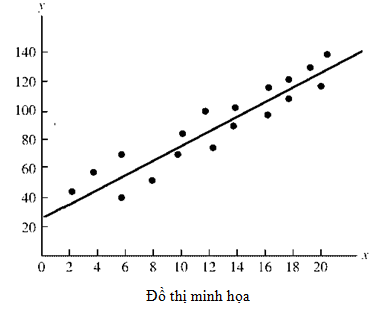
\includegraphics[width=\textwidth, height=0.4\textheight, keepaspectratio]{assets/linear_ex.png}
            \centering
        \end{figure}

        \item Như vậy đối với những dữ liệu có nhiều thuộc tính thì có thể mở rộng mô hình hồi quy tuyến tính như sau:
        \begin{equation}
            y = \theta_0 + \theta_1x_1 + \theta_2x_2 + ... + \theta_nx_n
        \end{equation}
    \end{itemize}

\subsection{Huấn luyện và kiểm tra mô hình}
    \begin{itemize}
        \item Để có thể tìm được mô hình phù hợp nhất cho bộ dữ liệu, bộ dữ liệu phải được chia thành 2 phần là \textbf{tập huấn luyện} và \textbf{tập kiểm tra}. Điều này sẽ giúp mô hình tránh được trường hợp \textbf{underfitting} và \textbf{overfitting}. Hai trường hợp này lần lượt là những mô hình quá tệ về độ chính xác của dữ liệu dự đoán hay mô hình quá phức tạp, cho kết quả rất tốt trên dữ liệu được cho nhưng lại quá kém so với dữ liệu khác ở thực tế. Tập huấn luyện \textbf{trainning set} sẽ được sử dụng để huấn luyện mô hình, còn tập kiểm tra \textbf{testing set} sẽ được sử dụng để kiểm tra mô hình đã được huấn luyện có tốt hay không. Tập kiểm tra sẽ được sử dụng để đánh giá mô hình.
    
        \item Trong thực tế đã nhiều phương pháp được dùng để  tạo ra tập \textbf{huấn luyện và kiểm tra}, trong đồ án này sẽ đề cập tới phương pháp \textbf{K-fold Cross Validation}.
        
        \subsubsection*{K-fold Cross Validation}\label{sec:k-fold-cross-validation}
            \begin{itemize}
                \item Theo như thông thường, chúng ta sẽ nghĩ tới việc chọn bao nhiêu phần để cho làm phần tập \textbf{huấn luyện}, và tập còn lại sẽ là tập \textbf{kiểm tra}. Tuy nhiên chúng ta sẽ không biết được 2 phần này nên chứa bao nhiêu dữ liệu trong từng trường hợp và nếu chia sai thì độ chính xác của mô hình sẽ chắc chắn không tốt. Chính vì vậy ý tưởng của phương pháp này chính là sẽ chia đều bộ dữ liệu này thành từng phần \textbf{fold} và sẽ thực hiện huấn luyện và kiểm tra từng phần để  tìm ra mô hình tốt nhất.
                \item Chi tiết các bước làm của phương pháp như sau: 
                    \begin{enumerate}
                        \item Chia bộ dữ liệu thành \textbf{k} phần bằng nhau.
                        \item Tại thời điểm xét từng phần dữ liệu, phần dữ liệu đó sẽ được chọn làm tập \textbf{kiểm tra}, và \textbf{k-1} còn lại sẽ được chọn làm tập \textbf{huấn luyện}.
                        \item Lưu lại độ chính xác của mô hình tại thời điểm đó.
                        \item Lặp lại các bước trên cho đến khi tất cả các phần dữ liệu đều được chọn làm tập \textbf{kiểm tra}.
                        \item Tính trung bình độ chính xác của các lần huấn luyện và kiểm tra và đây chính là độ chính xác của mô hình.
                    \end{enumerate}
                
                \begin{figure}[H]
                    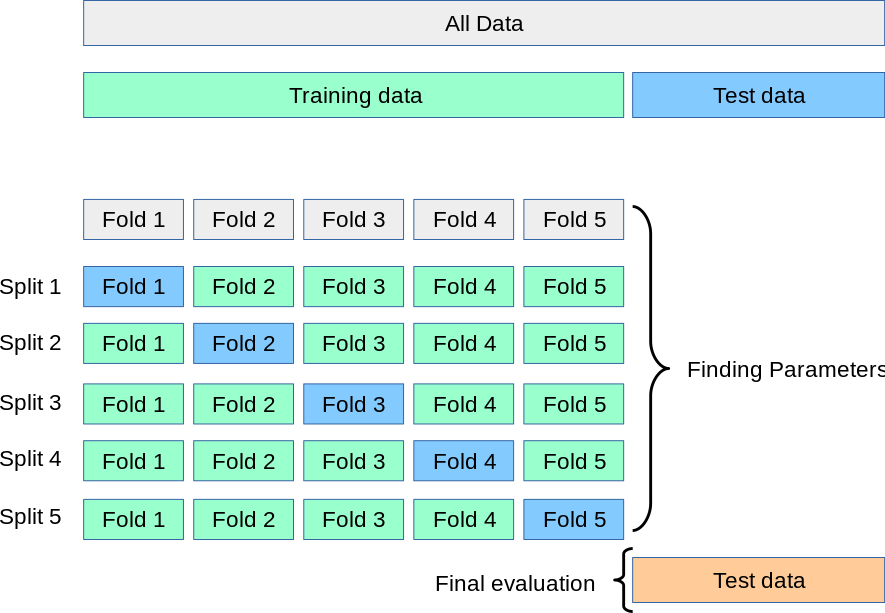
\includegraphics[width=\textwidth, keepaspectratio]{assets/grid_search_cross_validation.png}
                    \centering
                    \caption{Minh họa phương pháp K-fold Cross Validation}
                \end{figure}
                
            \end{itemize}
    \end{itemize}

\section{MÔ TẢ CÁC HÀM SỬ DỤNG}
\subsection{Lớp OLSLinearRegression}\label{sec:olslinearregression}
    Đây là lớp được cô \textbf{Phan Thị Phương Uyên} cung cấp, lớp này sẽ giúp sinh viên có thể xây dựng được mô hình hồi quy tuyến tính. Các thuộc tính của lớp này gồm:
    \begin{itemize}
        \item \textbf{fit(self, X, y)}: phương thức này sẽ thực hiện huấn luyện mô hình hồi quy tuyến tính với dữ liệu đầu vào là \textbf{X (dữ liệu đặc trưng)} và \textbf{y (dữ liệu mục tiêu)}. Hàm sẽ thực hiện và trả về trọng số của mô hình tương ứng với các đặc trưng theo công thức:
        \begin{equation}
            \theta = (X^TX)^{-1}X^Ty
        \end{equation}

        \item \textbf{get\_params()}: phương thức \textit{getter} sẽ trả về các trọng số của mô hình.
        
        \item \textbf{predict(self, X)}: phương thức này sẽ thực hiện dự đoán giá trị mục tiêu dựa trên dữ liệu đầu vào là \textbf{X (dữ liệu đặc trưng)} và trọng số của mô hình. Hàm sẽ thực hiện và trả về giá trị dự đoán theo công thức:
        \begin{equation}
            y = \theta_1x_1 + \theta_2x_2 + ... + \theta_nx_n
        \end{equation}
    \end{itemize}

\subsection{Lớp VarianceThreshold}
Đây là lớp được cung cấp bởi thư viện \textbf{sklearn.feature\_selection}, lớp này sẽ giúp có thể loại bỏ các đặc trưng có \textbf{phương sai} nhỏ hơn ngưỡng được đặt trước, cụ thể là:
    \begin{itemize}
        \item \textbf{VarianceThreshold(threshold)}: phương thức khởi tạo lớp, \textbf{tham số truyền vào} sẽ là ngưỡng để loại bỏ các đặc trưng có phương sai nhỏ hơn ngưỡng này.
        \item \textbf{fit(X\_train)}: phương thức sẽ thực hiện tính giá trị phương sai của các đặc trưng trong \textbf{X\_train}.
        Hàm loại bỏ các đặc trưng có phương sai nhỏ hơn ngưỡng \textbf{threshold} được đặt trước.Phương thức sẽ \textbf{không trả về giá trị nào} nhưng sẽ loại bỏ các đặc trưng có phương sai nhỏ hỡn ngưỡng của bộ dữ liệu đã được truyền vào.
    \end{itemize}
\subsection{Lớp mutual\_info\_regression}
    Đây là lớp được cung cấp bởi thư viện \textbf{sklearn.feature\_selection} được dùng để tính toán độ tương quan giữa các đặc trưng và mục tiêu, trong đó:
    \begin{itemize}
        \item \textbf{mutual\_info\_regression(X, y)}: phương thức khởi tạo lớp, \textbf{tham số truyền vào} sẽ là \textbf{ma trận các đặc trưng} và \textbf{vector mục tiêu}.Giá trị \textbf{trả về} của phương thức là mảng chứa các giá trị \textbf{mutual information} tương ứng với các đặc trưng.
    \end{itemize}

\subsection{Lớp SelectPercentile}
    Đây là lớp được cung cấp bởi thư viện \textbf{sklearn.feature\_selection}, lớp này khi sử dụng \textbf{phương thức khởi tạo SelectPercentile} thì cần truyền vào \textbf{phương thức tính độ tương quan} giữa các đặc trưng và mục tiêu, và \textbf{phần trăm} các đặc trưng muốn chọn. Giá trị \textbf{trả về} của phương thức là mảng chứa các đặc trưng có độ tương quan cao nhất với mục tiêu.

\subsection{Hàm mae(y\_pred, y\_test)}\label{sec:mae}
    Đây là hàm được cô \textbf{Phan Thị Phương Uyên} cung cấp, tham số truyền vào sẽ là \textbf{giá trị/tập giá trị dự đoán và giá trị/tập giá trị kiểm tra}. Hàm sẽ \textbf{trả về giá trị thể hiện độ chính xác} của giá trị được dự đoán, giá trị càng thấp thì độ chính xác càng cao. Công thức để tính độ chính xác là:
    \begin{equation}
        MAE = \frac{1}{n}\sum_{i=1}^{n}|y_{pred} - y_{test}|
    \end{equation}


\subsection{Hàm getTrain(index, folks)}\label{sec:getTrain}
    Đây là hàm hỗ trợ cho việc xác định tập dữ liệu \textbf{huấn luyện} trong phương pháp \hyperref[sec:k-fold-cross-validation]{\underline{K-fold Cross Validation}}. Giá trị đầu vào sẽ là \textbf{index} của phần dữ liệu đang xét và \textbf{folks} là tập dữ liệu đã được chia. Hàm sẽ \textbf{trả về tập dữ liệu huấn luyện}.

\subsection{Hàm Best\_Feature\_Personality(Df\_np, k\_cluster)}
    Đây là hàm giúp tìm ra đặc trưng tính cách tốt nhất trong 5 tính cách ở yêu cầu \textbf{2} trong phần \hyperref[sec:requirement]{\underline{YÊU CẦU ĐỒ ÁN}}. Giá trị đầu vào sẽ là \textbf{Df\_np} là tập dữ liệu đã được chuyển thành dạng \textbf{numpy array} và \textbf{k\_cluster} là số lượng cụm cần phải chia. Hàm sẽ thực hiện huấn luyện từng đặc trưng tính cách trên từng phần và sau cùng \textbf{trả về số thứ tự của đặc trưng tính cách tốt nhất}.Việc chọn ra đặc trưng tốt nhất sẽ được thực hiện dựa trên so sánh \textbf{MAE trung bình} của từng đặc trưng sau khi huấn luyện trên từng \textbf{k\_cluster} phần dữ liệu.

\subsection{Hàm best\_personality\_feature\_model()}\label{sec:bestpersonalityfeaturemodel}
    Đây là hàm sẽ thực hiện huấn luyện mô hình theo đặc trưng tốt nhất mà được tìm thấy ở hàm \textbf{Best\_Feature\_Personality}. Tham số truyền vào sẽ không có, nhưng giá trị trả về của hàm lần lượt 2 giá trị/tập giá trị \textbf{dự đoán} và \textbf{kiểm tra}.

\subsection{Hàm Best\_Feature\_Skill(Df\_np, k\_cluster)}\label{sec:BestFeatureSkill}
    Đây là hàm giúp tìm ra đặc trưng kĩ năng tốt nhất trong 3 kĩ năng ở yêu cầu \textbf{3} trong phần \hyperref[sec:requirement]{\underline{YÊU CẦU ĐỒ ÁN}}. Giá trị đầu vào sẽ là \textbf{Df\_np} là tập dữ liệu đã được chuyển thành dạng \textbf{numpy array} và \textbf{k\_cluster} là số lượng cụm cần phải chia. Hàm sẽ thực hiện huấn luyện từng đặc trưng kĩ năng trên từng phần và sau cùng \textbf{trả về số thứ tự của đặc trưng kĩ nang9 tốt nhất}.Việc chọn ra đặc trưng tốt nhất sẽ được thực hiện dựa trên so sánh \textbf{MAE trung bình} của từng đặc trưng sau khi huấn luyện trên từng \textbf{k\_cluster} phần dữ liệu.

\subsection{Hàm best\_skill\_feature\_model()}\label{sec:bestskillfeaturemodel}
    Đây là hàm sẽ thực hiện huấn luyện mô hình theo đặc trưng tốt nhất mà được tìm thấy ở hàm \textbf{Best\_Feature\_Skill}. Tham số truyền vào sẽ không có, nhưng giá trị trả về của hàm lần lượt 2 giá trị/tập giá trị \textbf{dự đoán} và \textbf{kiểm tra}.

\subsection{Hàm cross\_validation\_model(Df\_np, k\_cluster)}
    Đây là hàm sẽ thực huấn luyện để tìm ra độ chính xác của mô hình nhờ phương pháp \textbf{K-fold Cross Validation}. Về ý tưởng, cách thức cài đặt sẽ khá giống với hàm \textbf{Best\_Feature\_Personality} và \textbf{Best\_Feature\_Skill}, nhưng hàm này sẽ thực hiện huấn luyện trên tất cả các đặc trưng trong mảng \textbf{Df\_np} truyền đầu vào cùng với số nhóm muốn dữ liệu được chia và \textbf{trả về độ chính xác của mô hình}.

\subsection{Hàm model\_variance\_Dropping(X\_train)}\label{sec:droping-constant-feature}
    Đây là hàm sẽ hỗ trợ cho phương pháp xây dưng mô hình trong yêu cầu \textbf{3} trong phần \hyperref[sec:requirement]{\underline{YÊU CẦU ĐỒ ÁN}}, với tên gọi: \hyperref[sec:dropping-constant-feature]{\underline{Dropping Constant Feature}}, dựa trên giá trị \textbf{phương sai} của các đặc trưng. Tham số truyền vào sẽ là \textbf{X\_train} là tập dữ liệu huấn luyện của các đặc trưng không phụ thuộc. Hàm sẽ thực hiện \textbf{tìm ra các đặc trưng có phương sai lớn hơn ngưỡng} và \textbf{trả về tên các đặc trưng đó}.

\subsection{Hàm model\_correlation\_Dropping(X\_train, threshold)}
    Đây là hàm sẽ hỗ trợ cho phương pháp xây dưng mô hình trong yêu cầu \textbf{4} trong phần \hyperref[sec:requirement]{\underline{YÊU CẦU ĐỒ ÁN}},với tên gọi: \hyperref[sec:dropping-correlation-feature]{\underline{Dropping high-correlation Feature}}, dựa trên giá trị \textbf{phương sai} của các đặc trưng. Tham số truyền vào sẽ là \textbf{X\_train} là tập dữ liệu huấn luyện của các đặc trưng không phụ thuộc và mức độ tương quan mong muốn giữa các đặc trưng mong. Hàm sẽ thực hiện \textbf{chọn ra các đặc trưng có mức độ tương quan lớn hơn \textbf{threshold}} và \textbf{trả về tên các đặc trưng đó}.

\subsection{Hàm model\_MutualInfor\_selection(X\_train, Y\_train)}
    Đây là hàm sẽ hỗ trợ cho phương pháp xây dưng mô hình trong yêu cầu \textbf{4} trong phần \hyperref[sec:requirement]{\underline{YÊU CẦU ĐỒ ÁN}},với tên gọi: \hyperref[sec:selecting-MI-feature]{\underline{Selecting high-MI Feature}}, dựa trên giá trị \textbf{mutual information} của các đặc trưng. Tham số truyền vào sẽ là \textbf{X\_train} là tập dữ liệu huấn luyện của các đặc trưng không phụ thuộc và \textbf{Y\_train} là tập dữ liệu của đặc trưng phụ thuộc. Hàm sẽ thực hiện \textbf{chọn ra các đặc trưng có mức độ liên quan tới đặc trưng phụ thuộc cao} và \textbf{trả về  tên các đặc trưng đó}.

\subsection{Hàm my\_best\_model(models)}
    Đây là hàm sẽ tìm model nào tốt nhất từ mảng các \textbf{models} truyền vào qua phương pháp \textbf{K-fold Cross Validation}. Hàm sẽ \textbf{trả về số thứ tự của model tốt nhất trong mảng}.

\subsection{Hàm train\_my\_best\_model()}
    Đây là hàm huấn luyện model tốt nhất mà đã tìm được. \textbf{Đầu vào} của  hàm sẽ không có tham số, nhưng hàm sẽ \textbf{trả về giá trị/tập giá trị của dữ liệu phụ thuộc được dự đoán và kiểm tra}.

\section{KẾT QUẢ CỦA CÁC YÊU CẦU}
    \subsection{Yêu cầu 1}
        \subsubsection{Các bước thực hiện}
            \begin{enumerate}
                \item Truy xuất dữ liệu của 11 cột đặc trưng được yêu cầu (11 cột đầu tiên) trong tập huấn luyện và tập kiểm tra.
                \item Truy xuất cột Salary - là cột mục tiêu trong tập huấn luyện và tập kiểm tra.
                \item Tìm trọng số của mô hình hồi quy tuyến tính bằng cách sử dụng phương thức \textbf{fit} của lớp \hyperref[sec:olslinearregression]{\textbf{OLSLinearRegression}} với dữ liệu đầu vào là tập huấn luyện của 11 đặc trưng yêu cầu và đặc trưng mục tiêu Salary.
                \item Sử dụng phương thức \textbf{predict} của lớp \hyperref[sec:olslinearregression]{\textbf{OLSLinearRegression}} để dự đoán giá trị mục tiêu của tập kiểm tra.
                \item Sử dụng hàm \hyperref[sec:mae]{\textbf{mae}}  để tính độ chính xác của mô hình.
            \end{enumerate}

        \subsubsection{Công thức cho mô hình hồi quy (trọng số làm tròn tới 3 chữ số thập phân) và kết quả trên tập kiểm tra}
            \begin{itemize}
                \item     
                    \begin{align}
                        \begin{split}
                            \text{Salary} &= (-22756.513) \cdot X_1 + 804.503 \cdot X_2 + 1294.655 \cdot X_3 \\
                            &\quad + (-91781.898) \cdot X_4 + 23182.389 \cdot X_5 + 1437.549 \cdot X_6 \\
                            &\quad + (-8570.662) \cdot X_7 + 147.858 \cdot X_8 + 152.888 \cdot X_9 \\
                            &\quad + 117.222 \cdot X_{10} + 34552.286 \cdot X_{11}
                        \end{split}
                    \end{align}
                \item Độ chính xác của mô hình trên tập kiểm tra là: \textbf{104863.77754033315}
            \end{itemize}

    \subsection{Yêu cầu 2}
        \subsubsection{Các bước thực hiện}
        Cài đặt \hyperref[sec:bestpersonalityfeaturemodel]{\textbf{best\_personality\_feature\_model}} sẽ dùng để thực hiện yêu cầu 2 như sau:
            \begin{enumerate}
                \item Khởi tạo mảng chứa tên 5 đặc trưng tính cách vì trong bộ dữ liệu, 5 đặc trưng này đứng liên tiếp nhau.
                \item Thực hiện đổi chỗ ngẫu nhiên của cac dòng dữ liệu 1 lần.
                \item Gọi hàm \hyperref[sec:BestFeaturePersonality]{\textbf{Best\_Feature\_Personality}}  để tìm ra đặc trưng tốt nhất theo phương pháp \hyperref[sec:k-fold-cross-validation]{K-fold Cross Validation}.
                \begin{enumerate}
                    \item Thực hiện chia bộ dữ liệu huấn luyện thành 10 nhóm đều nhau (sử dụng hàm \textbf{numpy.array\_split}).
                    \item Thực hiện huấn luyện trên từng phần:
                        \begin{itemize}
                            \item Gọi hàm \hyperref[sec:getTrain]{\textbf{getTrain}} để lấy tập dữ liệu huấn luyện và tập kiểm tra là phần dữ liệu đang xét.
                            \item Với mỗi đặc trưng tính cách, thực hiện huấn luyện mô hình và tính độ chính xác của mô hình, lưu lại độ chính xác của mô hình trong mảng \textbf{mae\_arr}.
                        \end{itemize}
                    \item Sau khi xét hết phần dữ liệu, mảng \textbf{mae\_arr} thu được gồm 10 dòng và 5 cột tương đương với 10 phần dữ liệu được chia và 5 đặc trưng của mỗi dòng.
                    \item Tính độ chính xác trung bình của mỗi đặc trưng bằng cách lấy trung bình cộng của mỗi cột trong mảng \textbf{mae\_arr} và trả ra giá trị thứ tự của đặc trưng có \textbf{mae} nhỏ nhất. Một điều lưu ý là giá trị \textbf{mae trung bình} của mỗi đặc trưng sẽ thay đổi mỗi khi chạy chương trình vì việc đổi chỗ các dòng dữ liệu là ngẫu nhiên và khác nhau. 
                \end{enumerate}
                \item Sau khi tìm được đặc trưng tốt nhất, tiến hình truy xuất dữ liệu của đặc trưng đó để huấn luyện mô hình bằng cách sử dụng hàm \textbf{fit} của lớp \hyperref[sec:olslinearregression]{\textbf{OLSLinearRegression}}  và tính độ chính xác của mô hình bằng cách sử dụng hàm \hyperref[sec:mae]{\textbf{mae}}.
            \end{enumerate}
        
        \subsubsection{Kết quả tương ứng cho 5 mô hình từ k-fold Cross Validation}

    \begin{table}[H]
        \centering
        \resizebox{\textwidth}{!}{%
        \begin{tabular}{|c|c|c|}
        \hline
        \multicolumn{1}{|l|}{STT} & \multicolumn{1}{l|}{Mô hình với 1 đặc trưng} & MAE             \\ \hline
        1                         & conscientiousness                            & 306267.12993085 \\ \hline
        2                         & agreeableness                                & 300894.66699364 \\ \hline
        3                         & extraversion                                 & 307070.11566216 \\ \hline
        4                         & neuroticism                                  & 299387.84192331 \\ \hline
        5                         & openness\_to\_experience                     & 303008.96858233 \\ \hline
        \end{tabular}%
        }
    \end{table}

    \subsubsection{Kết quả tương ứng cho mô hình tốt nhất}
    \begin{itemize}
        \item Mô hình tốt nhất là mô hình đặc trưng \textbf{neuroticism} với độ chính xác trung bình là: \textbf{299387.84192331}
        \item Công thức hồi quy tuyến tính của mô hình tốt nhất: 
        \begin{equation}
            \text{Salary} = (-56546.304)*neuroticism
        \end{equation}
        \item Kết quả \textbf{mae} là: 291019.693226953
    \end{itemize}

    \subsubsection{Nhận xét}
    \begin{itemize}
        \item Kết quả của \textbf{k-fold Cross Validation} đã cho độ chính xác của đặc trưng \textbf{neuroticism} là tốt nhất, và kết quả này cũng đã được xác nhận qua các bài nghiên cứu thực tế. Theo bài nghiên cứu của trường đại học kinh tế \href{https://kse.ua/}{\textbf{Kyiv}} (ở Ukraine), 2 trong 5 tính cách có ảnh hưởng nhiều nhất tới mức lương của mỗi cá nhân đó là đức tính \textbf{hài lòng (agreeableness)} và \textbf{nhạy cảm trong cảm xúc(neuroticism)}.
        \item Trong đó, mức độ ảnh hưởng của sự nhạy cảm sẽ nhỉnh hơn một chút so với đức tính hòa thuận. Các dữ liệu được tiến hành nghiên cứu tại các nước như Đức, Anh, và Hà Lan ở \href{https://kse.ua/kse-research/relationship-between-your-personality-and-your-salary-level/}{đây} đã chỉ ra rằng: trong khi mức độ của sự hài lòng làm giảm từ 2-5\% mức lương ở Đức, hay 4-6\% ở Anh, thì mức độ nhạy cảm trong cảm xúc càng cao thì mức lương giảm khoảng 3\% ở Đức và 6\% ở Anh.
        \item Điều này cũng rất hợp lý vì những người có mức độ hài lòng cao sẽ có xu hướng ít phấn đấu để  cố gắng đạt mức lương cao hơn, hay người có sự không ổn định nhiều trong cảm xúc sẽ làm cho người đó luôn bị phân tâm, cảm thấy mệt mỏi, tiêu cực và điều này ảnh hưởng rất xấu tới công việc hay sự cố gắng của họ ở thời điểm đó. Chính vì vậy ngay trong bảng kết quả của \textbf{k-fold Cross Validation} đã cho thấy đặc trưng \textbf{neuroticism} và \textbf{agreeableness} có độ chính xác khá bằng nhau và \textbf{neuroticism} là tính cách có giá trị thấp hơn.
    \end{itemize}

\subsection{Yêu cầu 3}
    \subsubsection{Các bước thực hiện}
    Cài đặt \hyperref[sec:bestskillfeaturemodel]{\textbf{best\_skill\_feature\_model}} sẽ dùng để thực hiện yêu cầu 2 như sau:
        \begin{enumerate}
            \item Khởi tạo mảng chứa tên 3 đặc trưng kĩ năng để truy xuất các dữ liệu của 3 đặc trưng này.
            \item Thực hiện đổi chỗ ngẫu nhiên của cac dòng dữ liệu 1 lần.
            \item Gọi hàm \hyperref[sec:BestFeatureSkill]{\textbf{Best\_Feature\_Skill}}  để tìm ra đặc trưng tốt nhất theo phương pháp \hyperref[sec:k-fold-cross-validation]{K-fold Cross Validation}.
            \begin{enumerate}
                \item Thực hiện chia bộ dữ liệu huấn luyện thành 10 nhóm đều nhau (sử dụng hàm \textbf{numpy.array\_split}).
                \item Thực hiện huấn luyện trên từng phần:
                    \begin{itemize}
                        \item Gọi hàm \hyperref[sec:getTrain]{\textbf{getTrain}} để lấy tập dữ liệu huấn luyện và tập kiểm tra là phần dữ liệu đang xét.
                        \item Với mỗi đặc trưng tính cách, thực hiện huấn luyện mô hình và tính độ chính xác của mô hình, lưu lại độ chính xác của mô hình trong mảng \textbf{mae\_arr}.
                    \end{itemize}
                \item Sau khi xét hết phần dữ liệu, mảng \textbf{mae\_arr} thu được gồm 10 dòng và 3 cột tương đương với 10 phần dữ liệu được chia và 3 đặc trưng của mỗi dòng.
                \item Tính độ chính xác trung bình của mỗi đặc trưng bằng cách lấy trung bình cộng của mỗi cột trong mảng \textbf{mae\_arr} và trả ra giá trị thứ tự của đặc trưng có \textbf{mae} nhỏ nhất. Một điều lưu ý là giá trị \textbf{mae trung bình} của mỗi đặc trưng sẽ thay đổi mỗi khi chạy chương trình vì việc đổi chỗ các dòng dữ liệu là ngẫu nhiên và khác nhau. 
            \end{enumerate}
            \item Sau khi tìm được đặc trưng tốt nhất, tiến hình truy xuất dữ liệu của đặc trưng đó để huấn luyện mô hình bằng cách sử dụng hàm \textbf{fit} của lớp \hyperref[sec:olslinearregression]{\textbf{OLSLinearRegression}}  và tính độ chính xác của mô hình bằng cách sử dụng hàm \hyperref[sec:mae]{\textbf{mae}}.
        \end{enumerate}
    \subsubsection{Kết quả tương ứng cho 3 mô hình từ k-fold Cross Validation}
    \begin{table}[H]
        \centering
        \resizebox{\textwidth}{!}{%
        \begin{tabular}{|c|c|c|}
        \hline
        \multicolumn{1}{|l|}{STT} & \multicolumn{1}{l|}{Mô hình với 1 đặc trưng} & MAE        \\ \hline
        1                         & English                                      & 121837.9   \\ \hline
        2                         & Logical                                      & 120230.589 \\ \hline
        3                         & Quant                                        & 118051.624 \\ \hline
        \end{tabular}%
        }
    \end{table}

    \subsubsection{Kết quả tương ứng cho mô hình tốt nhất}
    \begin{itemize}
        \item Mô hình tốt nhất là mô hình đặc trưng \textbf{Quant} với độ chính xác trung bình là: \textbf{118051.624}
        \item Công thức hồi quy tuyến tính của mô hình tốt nhất: 
        \begin{equation}
            \text{Salary} = (585.895)*neuroticism
        \end{equation}
        \item Kết quả \textbf{mae} là: 106819.5776198967
    \end{itemize}

    \subsubsection{Nhận xét}
    \begin{itemize}
        \item Kết quả của đánh giá các mô hình từng kĩ năng đã cho thấy \textbf{kĩ năng định lượng (quantitative skill)} là đặc trưng tốt nhất trong 3 đặc trưng. Kĩ năng định lượng là kĩ năng đưa ra đánh giá, nhận xét một vấn đề nào đó dưới góc nhìn toán học, các thông số dữ liệu khổng lồ thể hiện dạng bảng, biểu đồ, đồ thị. Theo nghiên cứu của \href{https://www.journals.uchicago.edu/}{nhà xuất bản Đại học Chicago} ở \href{https://www.journals.uchicago.edu/doi/abs/10.1086/298239}{đây} đã cho rằng các kĩ năng, khả năng toán học là sự tạo ra khác biệt giữa mức độ thu nhập của mỗi người theo mô hình \href{https://www.open.edu/openlearn/mod/oucontent/view.php?id=67143&section=4}{Human Capital} (mô hình nghiên cứu về sự tăng trưởng kinh tế). Sự khan hiếm trong nhân lực có trình độ toán học cao sẽ làm cho mức lương của họ tăng lên có thể thấy ở các ngành nghề thực tế, đặc trưng nhất là \textbf{Data Science hay Data Analyst} - những ngành nghề đòi hỏi kĩ năng toán học cao.
        \item Chính vì sự cách biệt lớn giữa mức độ lương được tạo ra bởi kĩ năng định lương cho thấy kĩ năng này sẽ dự đoán được mức lương tốt hơn 2 kĩ năng còn lại là ngoại ngữ (tiếng anh) và kĩ năng suy nghĩ logic. Thêm vào đó, dựa vào hệ số mà mô hình được huấn luyện bởi đặc trưng định lượng là một hệ số dương, cho thấy mức lương sẽ tỉ lệ thuận với mức độ của đặc trưng này.
    \end{itemize}

\subsection{Yêu cầu 4}
Ở yêu cầu này sinh viên phải tự xây dựng các mô hình và chọn ra mô hình tốt nhất, chính vì thế dưới đây sẽ là phần nêu ra phương pháp và quá trình để chọn ra các mô hình. Tổng cộng có 3 mô hình được lựa chọn từ 3 phương pháp khác nhau, lần lượt là:
\begin{enumerate}
    \item Loại bỏ các đặc trưng có phương sai thấp.
    \item Loại bỏ các đặc trưng có mức độ tương quan cao.
    \item Chọn ra các đặc trưng có mức độ liên quan cao với đặc trưng mục tiêu.
\end{enumerate}
    \subsubsection{Lựa chọn mô hình}
        \paragraph{Mô hình 1: Loại bỏ các đặc trưng có phương sai thấp (dropping constant feature)}\label{sec:dropping-constant-feature}
    Mô hình đầu tiên được thực hiện theo phương pháp loại bỏ các \textbf{constant feature}. \textbf{Constant feature} là đặc trưng mà ở mỗi trạng thái (các dòng) hầu như đưa ra chỉ duy nhất 1 giá trị mà thôi. Giả sử ta có bộ dữ liệu như sau:
\begin{table}[h]
    \centering
    \resizebox{\columnwidth}{!}{%
    \begin{tabular}{|c|c|c|c|}
    \hline
    \multicolumn{1}{|l|}{Target} & \multicolumn{1}{l|}{Feature 1} & Feature 2  & \multicolumn{1}{l|}{Feature 3} \\ \hline
    1                            & 10                             & 1                            & 20                             \\ \hline
    2                            & 19                             & 1                            & 11                             \\ \hline
    3                            & 38                             & 1                            & 47                             \\ \hline
    \end{tabular}%
    }
    \end{table}\\
    Có thể thấy ở \textbf{feature 2}, dù cho trong trường hợp nào thì giá trị của đặc trưng này vẫn sẽ là \textbf{1}, lúc này feature 2 được gọi là \textbf{constant feature}. Việc giữ lại các đặc trưng này sẽ không có ý nghĩa gì vì chúng không đóng góp vào việc dự đoán mục tiêu. Chính vì vậy, ta sẽ loại bỏ các đặc trưng này đi.\\

    Để có thể loại bỏ các đặc trưng này thì sẽ xét giá trị \textbf{phương sai (variance)} của các đặc trưng. Variance là một đo lường cho mức độ biến đổi của các giá trị trong một tập dữ liệu và giá trị ấy được tính theo công thức:
    \begin{equation}
        Var(X) = \frac{1}{n}\sum_{i=1}^{n}(x_i - \overline{x})^2
    \end{equation}
    với $x_i$ là 1 trong những giá trị của đặc trưng \textbf{X} và $\overline{x}$ là giá trị trung bình của đặc trưng \textbf{X}.
    Khi tất cả các giá trị trong một feature đều giống nhau, không có sự thay đổi giữa chúng, do đó, variance của feature này là 0.\\

    Để có thể xác định các phương sai của các đặc trưng trong bộ dữ liệu, ta sẽ sử dụng hàm \textbf{var} của thư viện \textbf{pandas}, và giá trị phương sai của các đặc trưng có giá trị như sau: 

    \begin{figure}[H]
        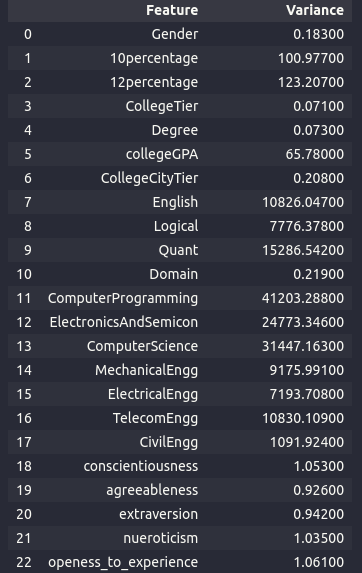
\includegraphics[width=\textwidth, height=0.5\textheight, keepaspectratio]{assets/variance.png}
        \centering
        \caption{Bảng giá trị phương sai của các đặc trưng}
    \end{figure}

    
    Dựa vào bảng phương sai của các đặc trưng, ta sẽ thực hiện loại bỏ các đặc trưng có giá trị phương sai nhỏ hơn 0.1 (các giá trị này có thể được tính xấp xỉ như bằng 0). Ta sẽ sử dụng lớp \hyperref[sec:library]{\textbf{VarianceThreshold}} với tham số  truyền vào phương thức khởi tạo là khoảng ngưỡng phương sai nhỏ nhất, và sử dụng phương thức \textbf{fit} của lớp này để loại bỏ các đặc trưng có phương sai nhỏ hơn ngưỡng này. Tất cả thao tác này được thực hiện trong hàm \hyperref[sec:droping-constant-feature]{\textbf{model\_variance\_dropping}}. \\
    
    Sau khi loại bỏ các đặc trưng này, ta sẽ thu được bộ dữ liệu mới với 22 đặc trưng như sau:
    \textbf{Gender, 10percentage, 12percentage, collegeGPA, CollegeCityTier, English, Logical, Quant, Domain, ComputerProgramming, ElectronicsAndSemicon, ComputerScience, MechanicalEngg, CivilEngg , TelecomEngg, ElectricalEngg, conscientiousness, agreeableness, extraversion, nueroticism, openess\_to\_experience}.        
    
    \pagebreak
        \paragraph{Mô hình 2: Loại bỏ các đặc trưng có mức độ tương quan cao (dropping high-correlation feature)}\label{sec:dropping-correlation-feature}
    Hệ số tương quan (\textbf{Correlation coefficient}) là giá trị thể hiện mức độ liên kết giữa 2 đặc trưng. Hệ số tương quan có giá trị nằm trong khoảng [-1, 1], với 1 là tương quan hoàn toàn, -1 là tương quan hoàn toàn nghịch đảo và 0 là không có tương quan. Vậy câu hỏi được đặt ra là: \textbf{Vì sao hệ số tương quan lại ảnh hưởng tới quá trình huấn luyện dữ liệu?}\\ 
    
    Đối với các mô hình hồi quy tuyến tính, một trong những giả định là các đặc trưng là độc lập tuyến tính với nhau. Nếu có sự tương quan giữa các đặc trưng, thì mô hình sẽ không thể xác định được đặc trưng nào là quan trọng hơn đặc trưng nào. Điều này sẽ làm cho mô hình không thể xác định được đặc trưng nào là quan trọng hơn đặc trưng nào, và dẫn tới việc mô hình sẽ không thể dự đoán được mục tiêu. Hiện tượng có các đặc trưng phụ thuộc vào nhau như vậy thì được gọi là hiện tượng \textbf{đa cộng tuyến (\href{https://en.wikipedia.org/wiki/Multicollinearity}{Multicollinearity})}.\\

    Thêm vào đó, điều này cũng đã được chứng minh dưới góc nhìn toán học như ở \href{https://www.quora.com/Why-is-it-important-to-remove-correlated-variables-when-performing-machine-learning-If-2-variables-are-correlated-how-do-you-choose-which-one-to-exclude-from-the-data-set}{đây}. Tóm tắt lại rằng giá trị trọng số được tính theo:
        \begin{equation}
            W_{LS} = (X^T  X)^{-1}  X^T  Y
        \end{equation}
    với $X$ là ma trận các đặc trưng, $Y$ là ma trận mục tiêu. Dưới góc nhìn của phân tích hồi quy, giá trị của biến độc lập $y$ sẽ được phân phối bởi giá trị phương sai \textbf{$\sigma^2$}, theo giả định này giá trị phương sai của trọng số sẽ là:
        \begin{equation}
            Var[W_{LS}] = \sigma^2 * (X^T X)^{-1} 
        \end{equation}
    Theo bài nghiên cứu đối với mô hình được ổn định thì giá trị phương sai của trọng số phải nhỏ. Nếu giá trị phương sai càng lớn thì có nghĩa là giá trị của trọng số cũng sẽ lớn trong mô hình huấn luyện, điều này sẽ dẫn tới việc mô hình sẽ không thể dự đoán được mục tiêu.

    Điều này được chứng minh thông qua \href{https://www.kaggle.com/code/phamdinhkhanh/singular-value-decomposition}{\textbf{phương pháp phân tích suy biến}}. Phương pháp này sẽ phân tích ma trận $X$ thành 3 ma trận $U, S, V$ sao cho:
        \begin{equation}
            X = U S V^T
        \end{equation}
    
    Như vậy, phương sai của của trọng số có thể  được viết lại như sau:
    \begin{align*}
        \begin{split}    
        \text{Var}[W_{LS}] &= \sigma^2 \cdot (X^T X)^{-1} \\
                            &= \sigma^2 \cdot (V S^T U^T U S V^T)^{-1} \\
                            &= \sigma^2 \cdot (V S^T S V^T)^{-1} \\
                            &= \sigma^2 \cdot V (S^T S)^{-1} V^T\\
                            &= \sigma^2 \cdot V S^{-2} V^T
        \end{split}
    \end{align*}
    Vì vậy khi giá trị tương quan cao, giá trị của ma trận "S" sẽ nhỏ, và khi nghịch đảo ma trận S thì giá trị của nó sẽ càng lớn. Điều này sẽ dẫn tới việc giá trị phương sai của trọng số sẽ càng lớn.   
    \\

    Để có thể xác định được các đặc trưng có mức độ tương quan cao với nhau thì ta sẽ sử dụng hàm \textbf{corr} của thư viện \textbf{pandas}. Bước đầu sẽ truy xuất tất cả cột thông tin của các đặc trưng ngoại trừ cột mục tiêu ("Salary"), tính hệ số tương quan và thể hiện giá trị tương quan của các đặc trưng dưới dạng biểu đồ heatmap như sau:
    \begin{figure}[H]
        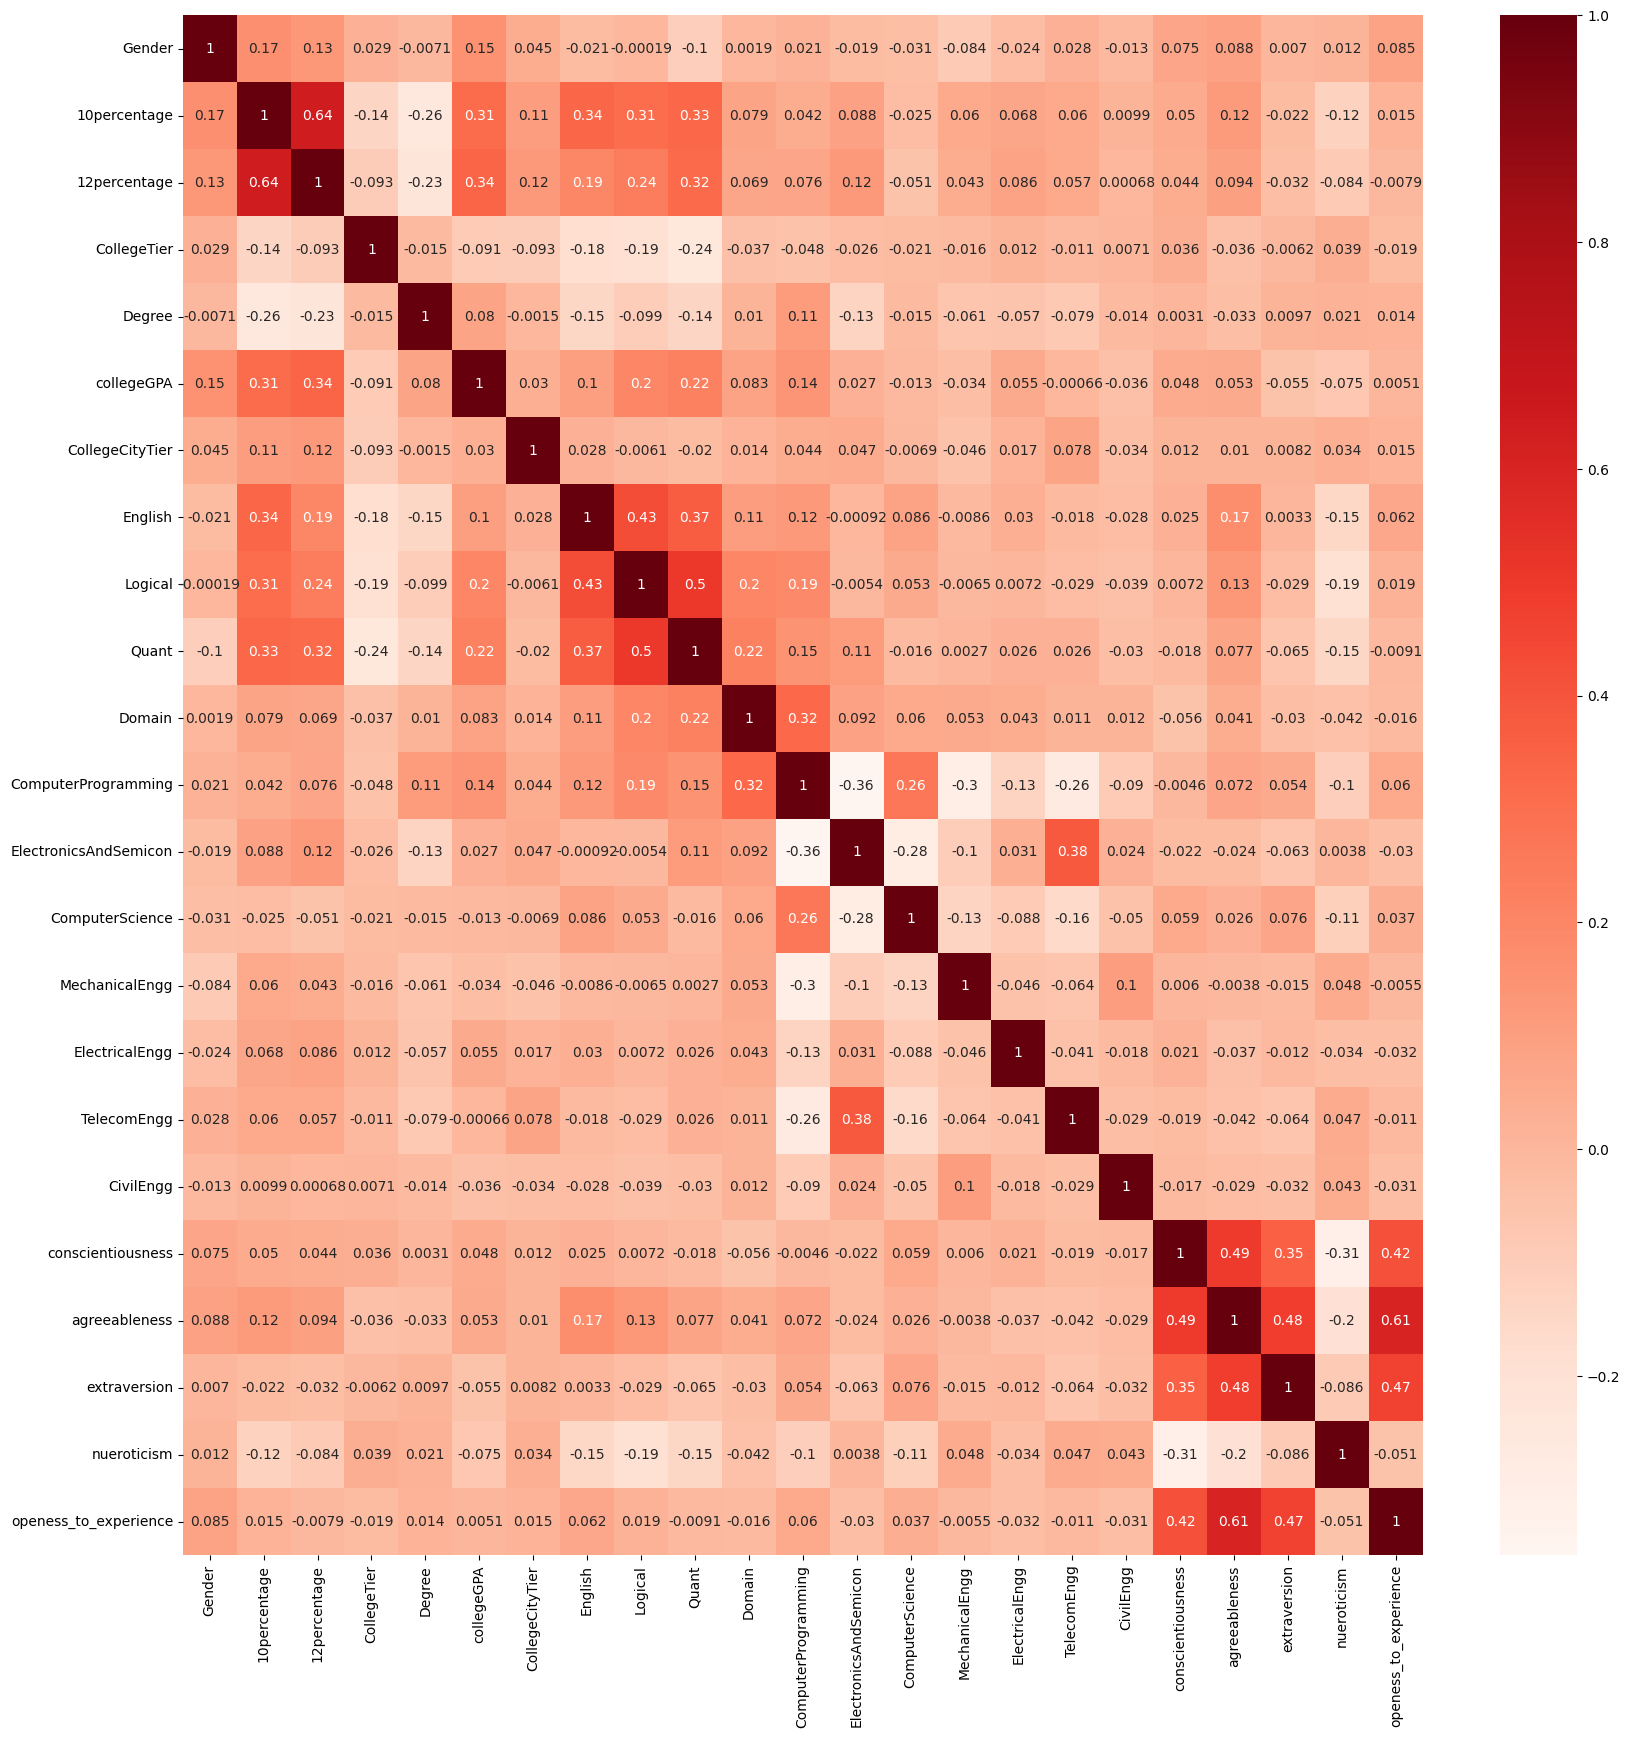
\includegraphics[width=\textwidth, keepaspectratio]{assets/heatmap.png}
        \centering
        \caption{Biểu đồ heatmap thể hiện mức độ tương quan của các đặc trưng}
    \end{figure}

    Theo nội dung của biểu đồ, ta có thể  giá trị hệ số  cao nhất là 0.64 giữa 2 đặc trưng \textbf{10percentage và 12percentage}, ta có thể đánh giá tổng quan rằng các đặc trưng có mức độ tương quan không quá cao, tuy nhiên ta vẫn sẽ tiến hành loại bỏ 1 trong 2 đặc trưng có \textbf{giá trị (không quan tâm tới dấu của giá trị)} hệ số tương quan lớn hớn hoặc bằng 0.6.\\
    
    Sau khi loại bỏ các đặc trưng này, ta sẽ thu được bộ dữ liệu mới với 21 đặc trưng để tạo mô hình 2 như sau: \textbf{Gender, 10percentage, CollegeTier, Degree, collegeGPA, CollegeCityTier, English, Logical, Quant, Domain,
    ComputerProgramming, ElectronicsAndSemicon, ComputerScience, MechanicalEngg, CivilEngg, ElectricalEngg, TelecomEngg, conscientiousness, agreeableness, extraversion, nueroticism}.

    \paragraph{Mô hình 3: Chọn ra các đặc trưng có mức độ liên quan cao với đặc trưng mục tiêu (selecting high-MI feature)}\label{sec:selecting-MI-feature}
    \newpage
\section{TÀI LIỆU THAM KHẢO}
\begin{itemize}
    \item Cô Phan Thị Phương Uyên.
    \item 
    \href{https://ie.nitk.ac.in/blog/2020/01/19/algorithms-for-adjusting-brightness-and-contrast-of-an-image/}{Công thức thay đổi độ sáng và độ tương phản}.

    \item
    \href{https://www.dfstudios.co.uk/articles/programming/image-programming-algorithms/image-processing-algorithms-part-5-contrast-adjustment/}{Thay đổi độ tương phản}.

    \item 
    \href{https://www.baeldung.com/cs/convert-rgb-to-grayscale}{Công thức chuyển thành hình xám}.

    \item 
    \href{https://dyclassroom.com/image-processing-project/how-to-convert-a-color-image-into-sepia-image}{Công thức chuyển thànhh hình màu sepia}.

    \item \href{https://en.wikipedia.org/wiki/Kernel_(image_processing)}{Công thức và ma trận các kernel để làm mờ và rõ nét ảnh}.

    \item 
    \href{https://www.youtube.com/watch?v=4Eh0y3LHTNU&t=658s}{Triển khai thuật toán cho làm mờ ảnh}.
    \item \href{https://www.maa.org/external_archive/joma/Volume8/Kalman/General.html}{Phương trình ellip}.

    \item \href{https://math.stackexchange.com/questions/2003517/how-to-calculate-width-and-height-of-a-45-rotated-ellipse-bounded-by-a-square}{Công thức của ellip khi xoay 45 độ}.

    \item \href{https://numpy.org/doc/stable/user/index.html#user}{Tài liệu các hàm trong thư viện numpy}.

    \item \href{https://matplotlib.org/stable/api/_as_gen/matplotlib.pyplot.imshow.html}{Thư viện matplotlib hỗ trợ xuất ảnh và lưu ảnh}.

    \item \href{https://pillow.readthedocs.io/en/stable/reference/Image.html}{Thư viện Pillow hỗ trợ đọc ảnh}.
    
\end{itemize}
% ========== END [MAIN CONTENT] ==========
\end{document}